\section{Woher bekomme ich KFlog, wie wird es installiert?}
KFlog ist ausschlie�lich im Internet �ber die Projekt-Homepage www.kflog.org zu beziehen.
Dort werden die verschiedenen Versionen des Programms und das notwendige Kartenmaterial zum Download bereitgestellt.
\\In der Regel sollte man sich den Quell-Code der letzten Version herunterladen.
\\Mit dem bekannten Linux-Dreisatz
\\ \\
\textit{./configure
\\make
\\make install}
\\
\\wird das Programm �bersetzt und installiert (f�r make install sollte man vorher Root-Rechte mit dem Befehl su erlangt haben).
\\F�r den versierten Anwender sollte der Befehl ./configure --help ausgef�hrt werden, damit die verschiedenen Optionen zur �bersetzung des Quellcodes ersichtlich werden.
\\Damit das Programm auch richtig arbeiten kann, sind noch verschiedene Daten �ber das Fluggebiet und eine Liste der Flugpl�tze von N�ten.
\\Diese speziellen Daten wie Luftraumstrukturen, St�dte, Stra�en, Gew�sser, Eisenbahnen usw. k�nnen ebenfalls von der Homepage im sog. Maproom heruntergeladen werden.
\\F�r diese Daten sind verschiedene Verzeichnisse vorgesehen. Als Voreinstellung gelten folgende Pfade:
\\
\begin{itemize}
\item f�r Liste der Flugpl�tze \$KDEDIR/share/apps/kflog/mapdata/airfields
\item f�r die Luftraumstrukturen \$KDEDIR/share/apps/kflog/mapdata/airspace
\item f�r die Terrain-Daten \$KDEDIR/share/apps/kflog/mapdata/
\end{itemize}

Diese Verzeichnisse werden mit der Installation automatisch angelegt und die entsprechenden Daten sind an diese Stellen zu kopieren (Diese Pfade k�nnen sp�ter aber auch noch im Einstellungs-Men� ge�ndert werden).
\\ \\ \textbf{Hinweis: Wenn die Dateien f�r die verschiedenen Daten vertauscht werden kommt es zu Abst�rzen des Programms und KFlog kann nicht ordentlich gestartet werden!!!}
\\ \\
Das Programm kann in der Konsole mit dem Befehl \textit{kflog} gestartet werden.
Nun sollte ein Startbild mit dem KFlog-Logo (s. Abb. 1) erscheinen und anschlie�end sollte das Programm mit dem Hauptfenster zu sehen sein (s. Abb. 2).
\\
\begin{figure}[htpb]
\begin{center}

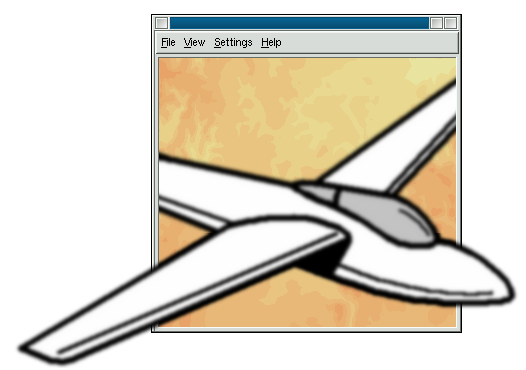
\includegraphics[scale=.3]{Bilder/fertig/splash.png} 

\\
\caption{Startbild}
\end{center}
\end{figure}
\begin{figure}[htpb]
\begin{center}
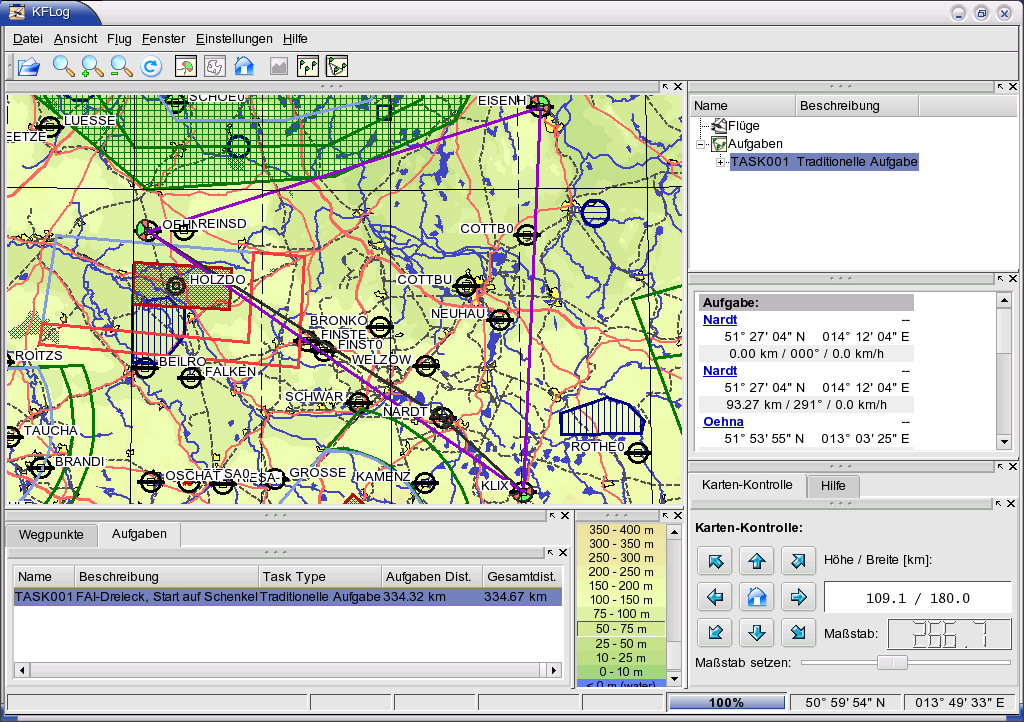
\includegraphics[scale=.34]{Bilder/fertig/Hauptfenster.png} 
\\
\caption{Hauptfenster von KFlog}
\end{center}
\end{figure}
